\documentclass[a4paper, 12pt]{article}
\usepackage{graphicx}
\usepackage[a4paper, top=2cm , bottom=2cm , right=2cm , left=2cm ]{geometry}
\usepackage{graphicx} % Required for inserting images
\usepackage[T1]{fontenc}
\usepackage[latin1]{inputenc}
\usepackage{glossaries}
\usepackage{graphicx}
\usepackage{amsfonts}
\usepackage[hidelinks]{hyperref}
\usepackage{pifont}
\usepackage{eufrak}
\usepackage{float}
\usepackage{verbatim}
\usepackage{amssymb}
\usepackage{listings}
\usepackage{amsthm}
\usepackage{matlab-prettifier}
\usepackage{pifont}
\usepackage{multicol}
\usepackage{verbatim}
\usepackage{tikz}
\usetikzlibrary{shapes,arrows}
\usepackage{tikz}
\tikzstyle{mybox} = [draw=black, thin, rectangle, rounded corners, inner ysep=5pt, inner xsep=5pt, fill=blue!15]
\newtheorem{theorem}{Theorem}

\usepackage[affil-it]{authblk}
\usepackage{cleveref}
\usepackage{booktabs} % To thicken table lines

\usepackage{amsthm}
\newtheorem*{remark}{Remark}
\newtheorem*{result}{Result}

\title{\textbf{Structured uncertainty and $\mu$-analysis}}


\author{Carlo Migliaccio
%\\Master's Degree in Computer Engineering\\
%Politecnico di Torino}
}
\date{December 2024}

\begin{document}
\maketitle

\section{Structured uncertainty}
Dealing with \textbf{structured uncertainty} and the analysis of feedback control systems affected by it, we are going to consider the \textit{general control configuration} depicted in the figure below.
Here $z_\Delta$ and $w_\Delta$ are the so-called \textit{uncertainty channels}, which in turn are the signals connecting the \textbf{uncertainty sources} with the known part of the feedback control system. On the other hand the signals $z_p$ and $w_p$ are chosen in order to satisfy \textbf{performance requirements} from which the name \textbf{performance channel}. In the following we deal with mainly with \textbf{parametric uncertainty}.


\begin{multicols}{2}
    \begin{center}
        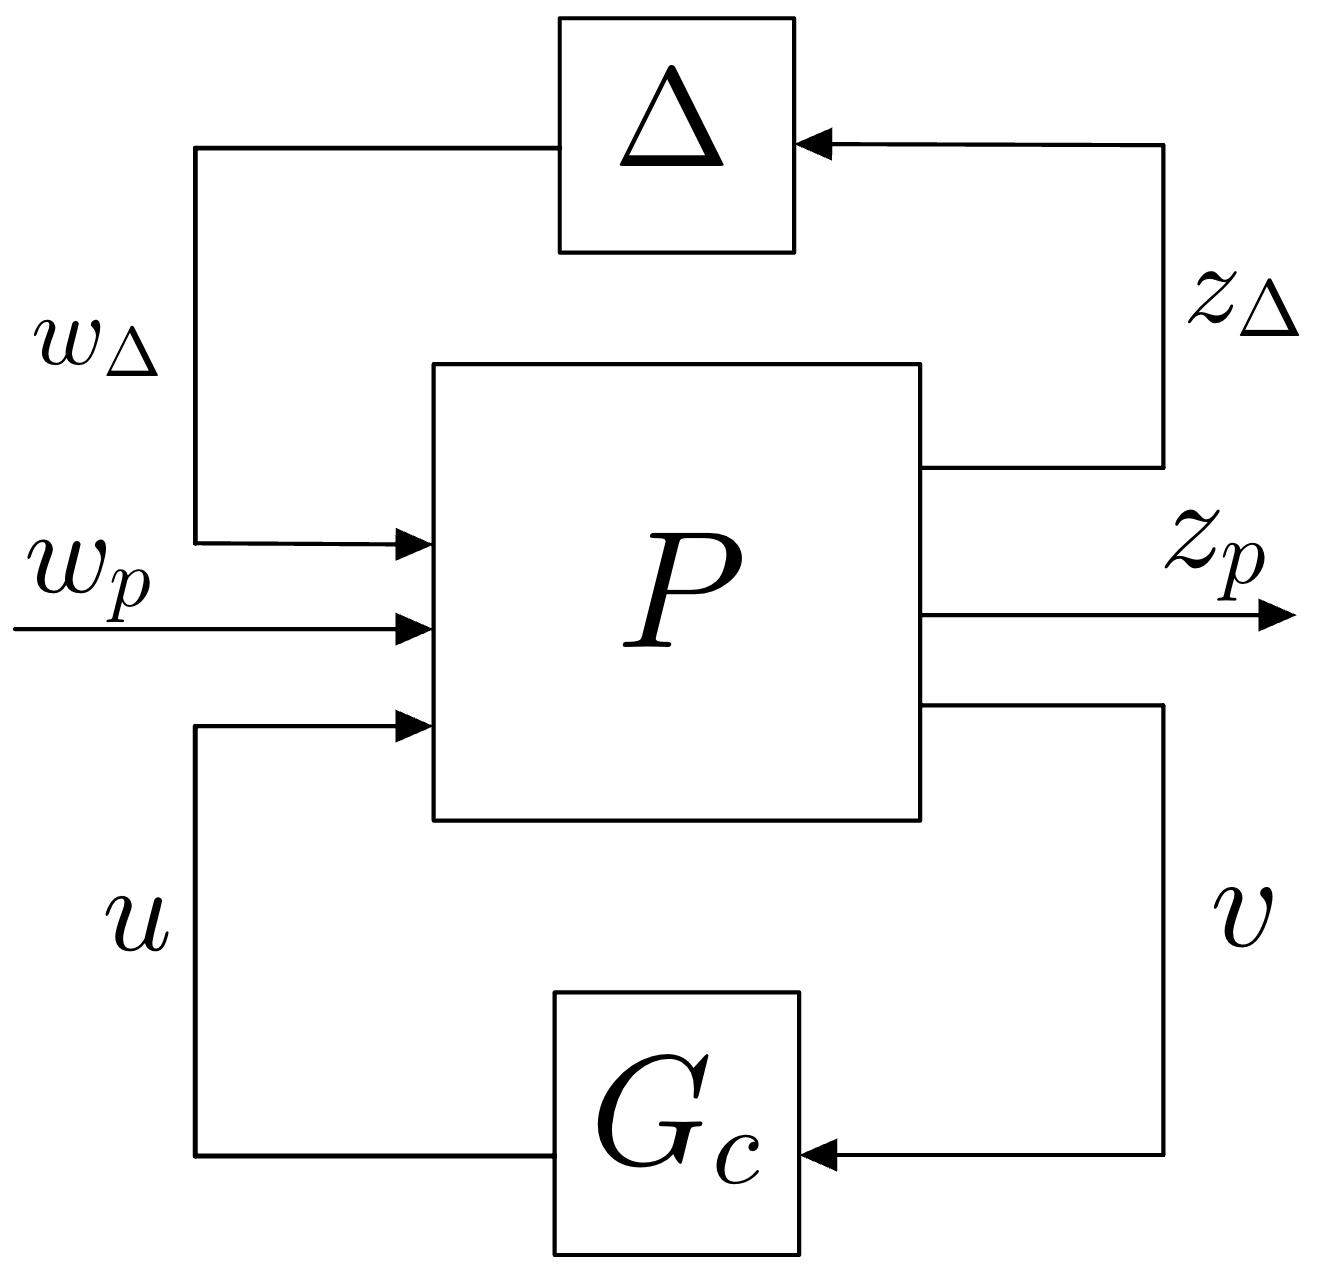
\includegraphics[scale=0.14]{img/pdg.jpg}\\
        $P\Delta{G_c}$ \textsf{general structure}
    \end{center}
    

\noindent
In such a general structure the sources of uncertainty $\Delta_i$ are pulled out to form a \textbf{block diagonal matrix} $\Delta$, that is:
\begin{equation}\label{eq:Delta_blocks}
    \Delta=\text{diag}\{\Delta_i\}=\begin{bmatrix}
        \Delta_1&0&\dots&0\\
        0&\Delta_2&\dots&0\\
        \vdots&\vdots&\ddots&\vdots\\
        0&\dots&0&\Delta_n
    \end{bmatrix}
\end{equation}
We will consider different sources of uncertainty (real, complex full mzatrix, real repeated real scalar values).
\end{multicols}

\subsection{Uncertainty sources}
In the analysis of stability and performances by using the $\mu$-analysis we will consider mainly:
\begin{itemize}
    \itemsep-0.2em
    \item \textbf{Real scalar} perturbations $\Delta_i\in\mathbb{R}$ such that $\vert \Delta_i \vert\le1$; 
    \item \textbf{Complex full matrix} perturbations $\Delta_i(s)\in\mathbb{C}^{m,m}$, $\Vert \Delta_i \Vert_\infty\le1$;
    \item \textbf{Repeated real scalar} perturbations $\Delta_i I_r$, where $I_r$ is an $r\times{r}$ identity matrix, and $\Delta_i\in\mathbb{R}$, $\Delta_i\le{1}$ 
\end{itemize}
In order to perform a computer-aided $\mu$-analysis, how we will see we use the command \texttt{mu} that among all of the parameters, take as input a matrix called \texttt{deltaset}. The main objective of such a matrix is \textit{describing the blocks of \Cref{eq:Delta_blocks}} ( the block diagonal matrix we mentioned) in term of: (i) type, (ii) dimensions, (iii) number of independent locations in which the uncertainty itself appears. By using a summarizing table, we mention the principal pattern we can find in analyzing our feedback control systems. 

\begin{table}[h!]
    \centering
    \begin{tabular}{p{7cm} p{5cm}}
        \toprule[1pt]
        \textbf{Type of $\Delta_i$}&\textbf{\texttt{deltaset} row}\\
        \midrule
        Scalar real parameter&$[-1\quad{1}]$ or $[-1\quad0]$\\
        \midrule
        $f$-repeated real parameter&$[-f\quad{0}]$\\
        \midrule
        Scalar $1\times1$ unmodeled dynamics&$[1\quad{1}]$ or $[1\quad0]$\\
        \midrule
        $r\times{c}$ full unmodeled dynamics&$[r\quad{c}]$\\        \bottomrule[1pt]
    \end{tabular}
    \caption{\texttt{deltaset} for describing $\Delta$}
    \label{tab:deltaset}
\end{table}
\noindent
Wheter in the feedback control system there are $U$ uncertainty sources the final matrix will be such that \texttt{deltaset} $\in\mathbb{R}^{U,2}$.
In the following sections we are going to do some examples which will clarify what is the structure of the \texttt{deltaset} matrix according to the structure of the uncertain plant $G_p(s)$.
The models can be considered for the uncertainty are the following, given the generic parameter $k$: 

\begin{table}[h]
    \centering
    \begin{tabular}{p{8cm} p{6cm}}
        \toprule[1pt]
        \textbf{MODEL SET}&\textbf{Mathematical description}\\
        \midrule
        \textsc{Additive uncertainty set}&$k=k_n+W_k{\Delta_k}, \ \vert \Delta_k \vert \le 1$  \\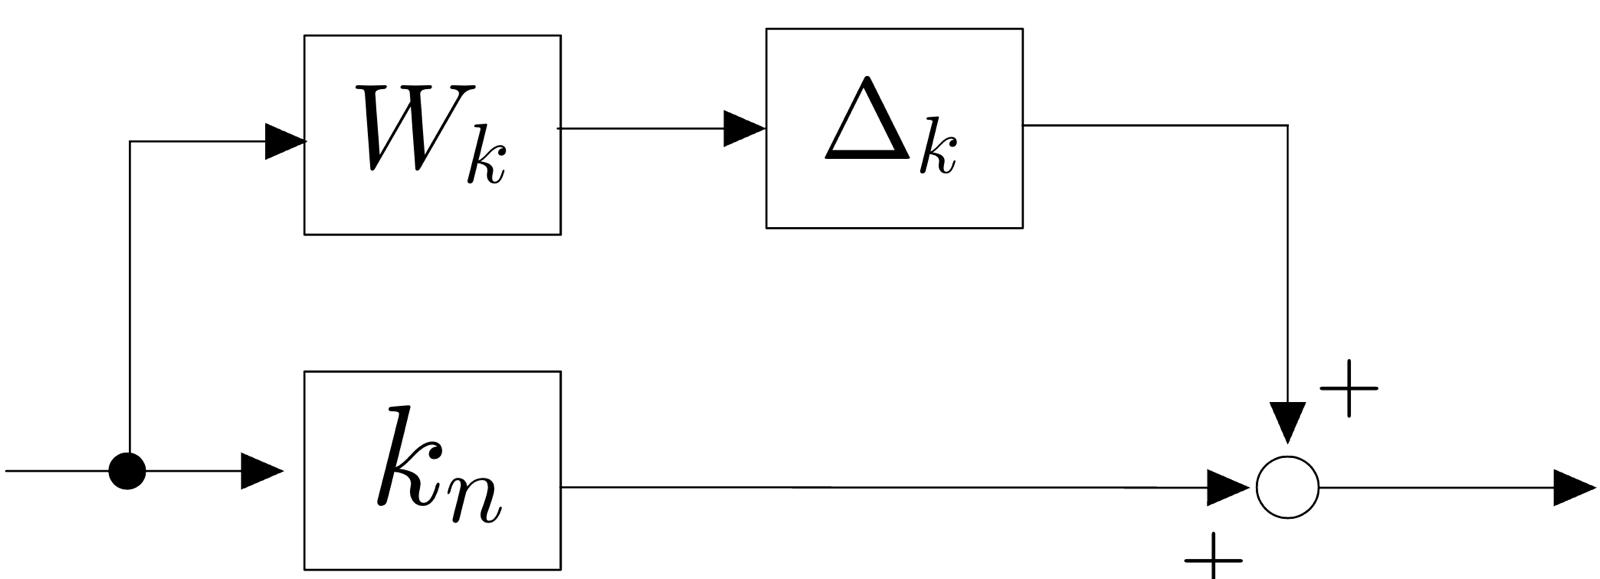
\includegraphics[scale=0.12]{img/add_k.jpg}\\
        \midrule
        \textsc{Multiplicative uncertainty set}&$k=k_n(1+W_k\Delta_k), \ \vert \Delta_k \vert \le1$ \\ 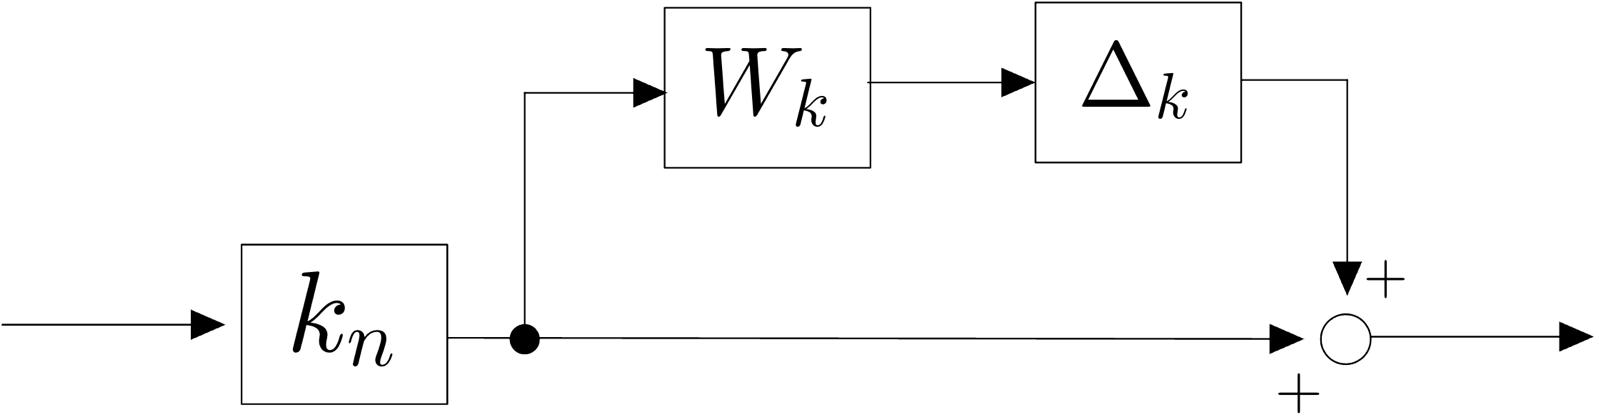
\includegraphics[scale=0.14]{img/mul_k.jpg}\\
        \bottomrule[1pt]
    \end{tabular}
    \caption{Uncertainty model sets}
    \label{tab:uncertainty_set}
\end{table}


\subsection{Fundamental bricks for structured uncertainty}
Going on to analyze the structure of our uncertain system we can find in the transfer function some fundamental bricks that put all together will give us the description through block diagrams of the uncertain plant. \textsf{Some aspects are presented in details for the first example while they are not repeated for the following ones which are using exactly the same steps.}

\subsubsection{Real Pole in zpk form}

\subsubsection*{Example 1 (pole in the feedback path)}
Given the following transfer function for an uncertain plant 
\begin{equation}\label{eq:ex1}
    G_p(s)=\frac{k}{s+p} \quad  
    \underline{k}\le {k} \le \overline{k}, \quad
    \underline{p}\le {p} \le \overline{p}
\end{equation}
we want to obtain its block diagram description. In particular for each parameter is required to obtain the central estimate $k_n$ and $p_n$ and the radius of uncertainty $W_k$ and $W_p$. Compute also the matrix $\Delta$ and the associated \texttt{deltaset} for the command \texttt{mu}.\\
The first step is for computing the value $k_n$, $p_n$, $W_k$ and $W_p$:
\begin{align}
    k_n=\frac{\underline{k}+\overline{k}}{2} \quad
    W_k=\frac{\overline{k}-\underline{k}}{2}, \qquad 
    p_n=\frac{\underline{p}+\overline{p}}{2} \quad
    W_p=\frac{\overline{p}-\underline{p}}{2}
\end{align}
\noindent
At the end of the day, we are likely to build such block diagrams in \textsc{Simulink}\footnote{
    Some algebraic manipulation are needed in order to avoid non proper blocks that -- for sure-- are going to raise an error during the simulation.
}, for this reason we have to manipulate the expression of \Cref{eq:ex1} in order to be able to represent them. If we put in evidence $s$ at the denominator we can write:

\begin{multicols}{2}
    {\large{
        \begin{equation*}
            G_p(s)=\frac{k}{s(1+\frac{p}{s})}=k \frac{\frac{1}{s}}{1+\frac{p}{s}}
        \end{equation*}
    }}
    The first term of the expression is simply a gain, while we can see the second term as a \textit{feedback configuration} with negative feedback.
    \newcolumn 
    \begin{center}
        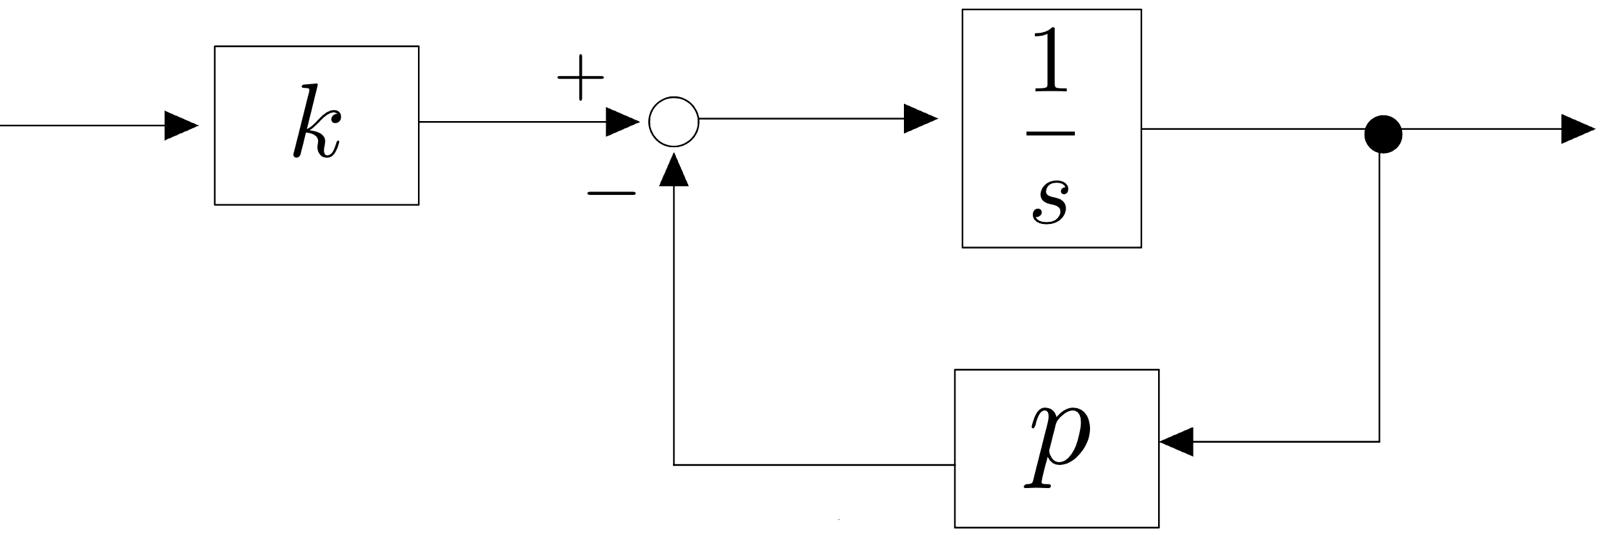
\includegraphics[scale=0.15]{img/ex1.jpg}\\
        \textsf{Block diagram for \Cref{eq:ex1}}
    \end{center}
\end{multicols}

\noindent
\textsf{\large \textbf{Additive Uncertainty Set}}\\
If we use the as uncertainty set the \textit{additive one} the block diagram we have showed changes as follows: 

\begin{figure}[h]
    \centering
    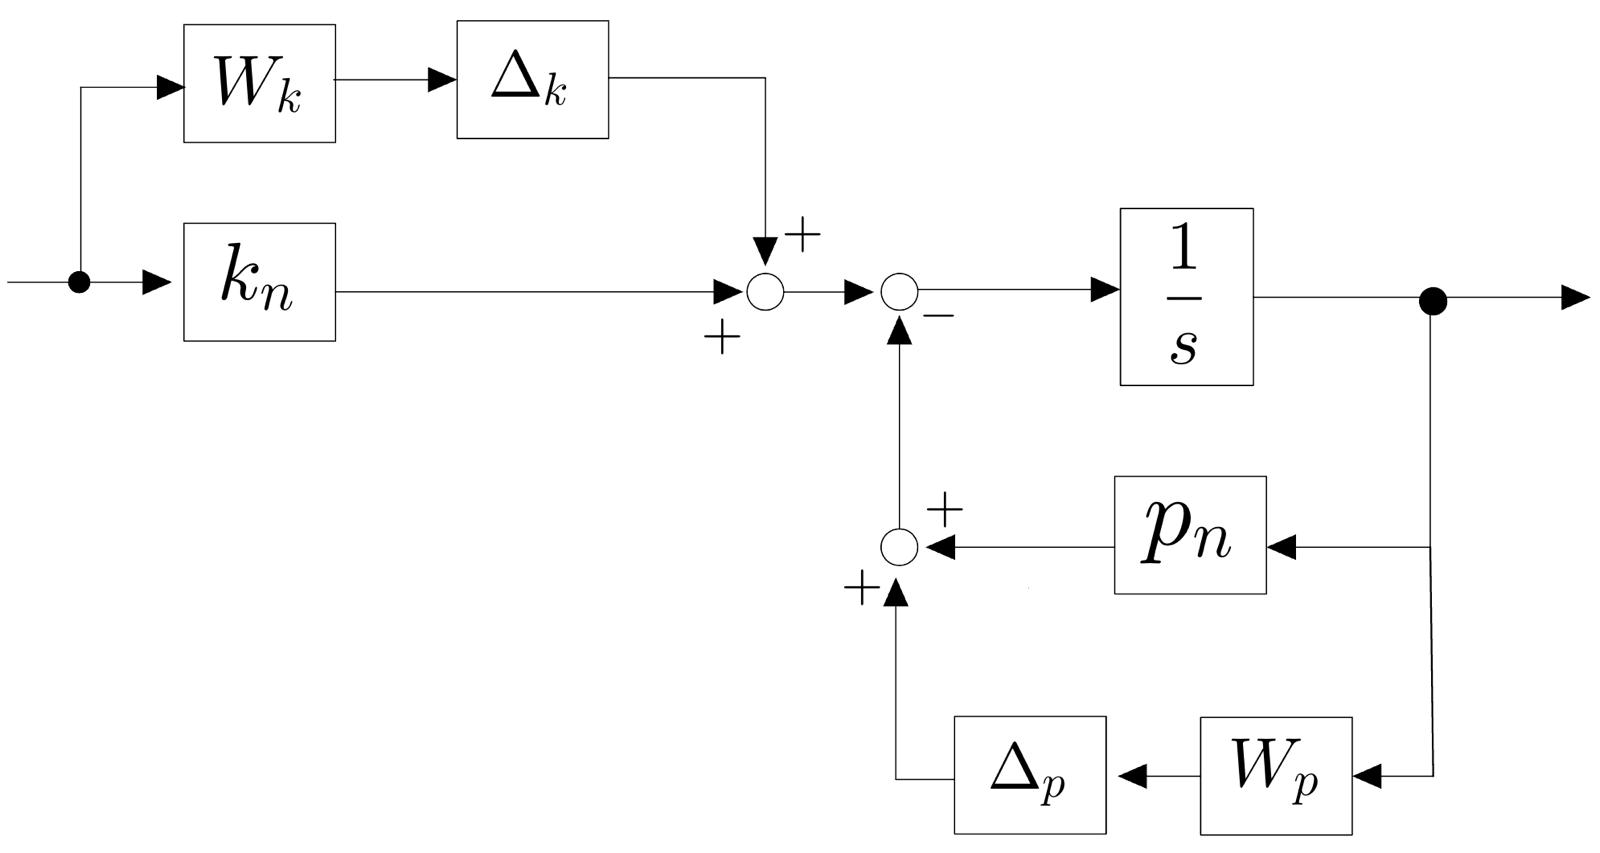
\includegraphics[scale=0.23]{img/ex1_add.jpg}
    \caption{Block diagram of $G_p(s)$ (additive model)}
\end{figure}
\noindent
Note that we have only added the for the parameters the uncertain description as indicated in \Cref{tab:uncertainty_set}. With the objective of obtaining the the $P\Delta{G_c}$ structure we have to: (i) put such a diagram in the Feedback control System (FCS) scheme; (ii) pull out all of the $\Delta_i$ blocks; (iii) pull out the controller $G_c$. \\
More interesting is the construction of the matrix $\Delta$ and its describing matrix \texttt{deltaset}. For this aim is crucial that all of the uncertainty channels are properly numbered. The block diagram becomes the one in \Cref{fig:ex1_num}, where there are also the signals entering/coming from the (structured) uncertainty block $\Delta$. According to the numbering we use in the block diagram we have to insert the diagonal blocks into $\Delta$ as reported here:

\begin{equation}
    \Delta=\begin{bmatrix}
        {\color{red}{\Delta_k}}&0\\
        0&{\color{blue}{\Delta_p}}
    \end{bmatrix} \qquad
    \texttt{deltaset}=[
        \underbrace{\texttt{{\color{red}{-1,1}}}}_{\color{red}1}; 
        \underbrace{\texttt{{\color{blue}-1,1}}}_{\color{blue}2}]
\end{equation}

\begin{figure}[h]
    \centering
    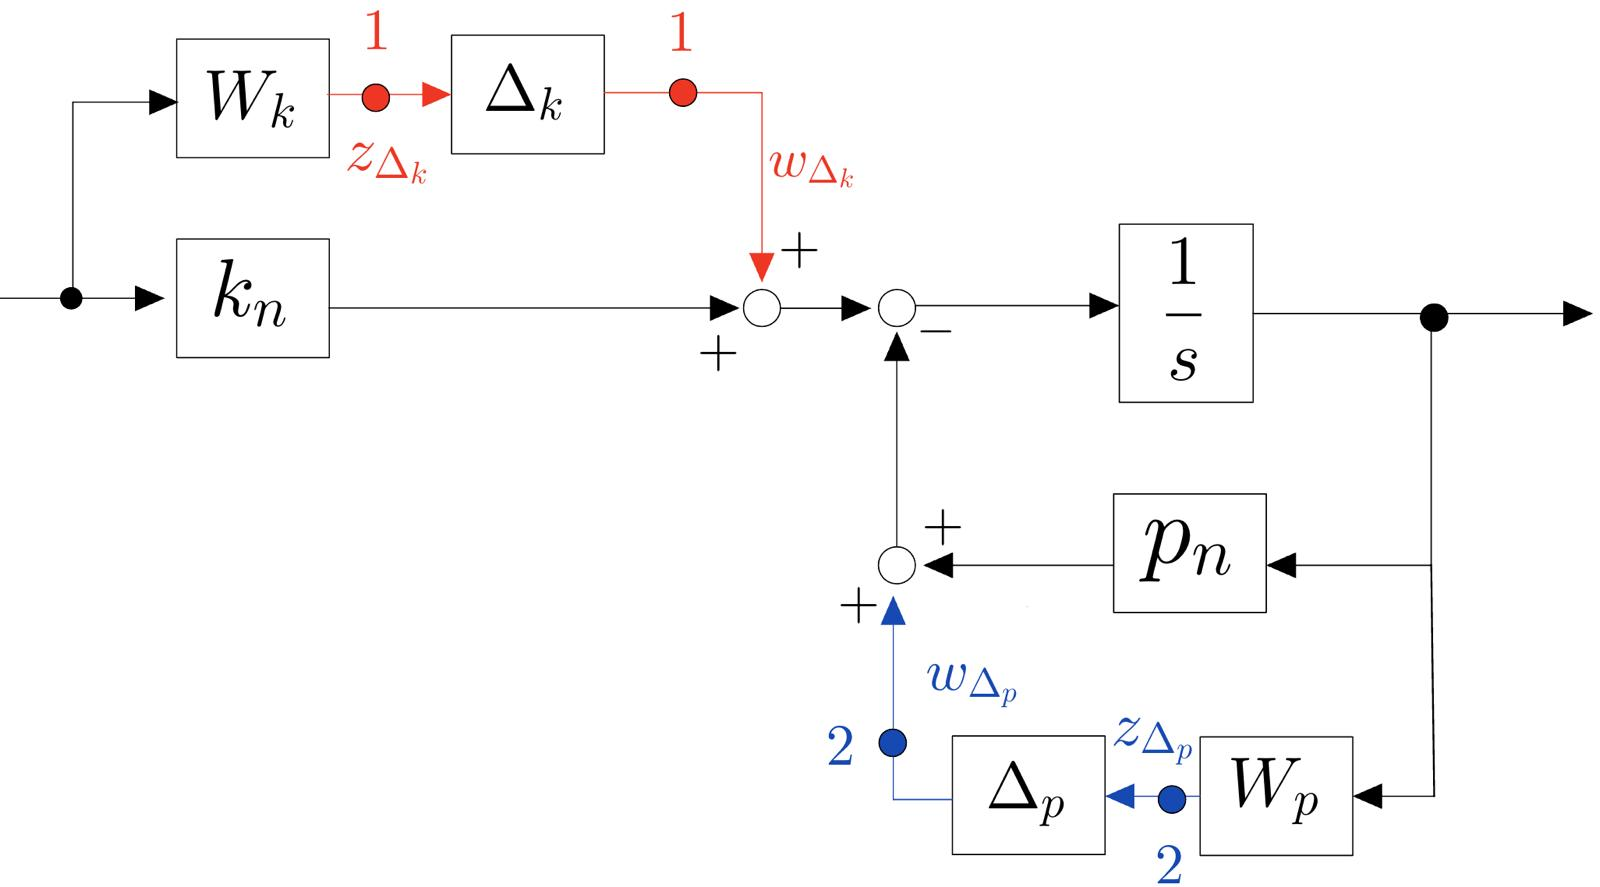
\includegraphics[scale=0.23]{img/ex1_num.jpg}
    \caption{Block diagram of $G_p(s)$ (additive) with numbered sources}
    \label{fig:ex1_num}
\end{figure}


\noindent
The first block of $\Delta$ is the one related to the uncertain parameter $\color{red} k$, the second the one related to the uncertain parameter $\color{blue} p$. Let the colors guide you in the understanding the relationship existing between the block diagram and related $\Delta$ and \texttt{deltaset}.\\

\noindent
\textsf{\large \textbf{Multiplicative Uncertainty Set}}\\
Identical reasoning can be done, if we assume to take as model of uncertainty the \textit{multiplicative one}. Substituting in the general scheme, the structure for the uncertain parameters from the \Cref{tab:uncertainty_set}, the scheme in \Cref{fig:ex1_mul} is obtained. The associated matrix $\Delta$ and the \texttt{deltaset} array are the same as before.

\begin{figure}[h]
    \centering
    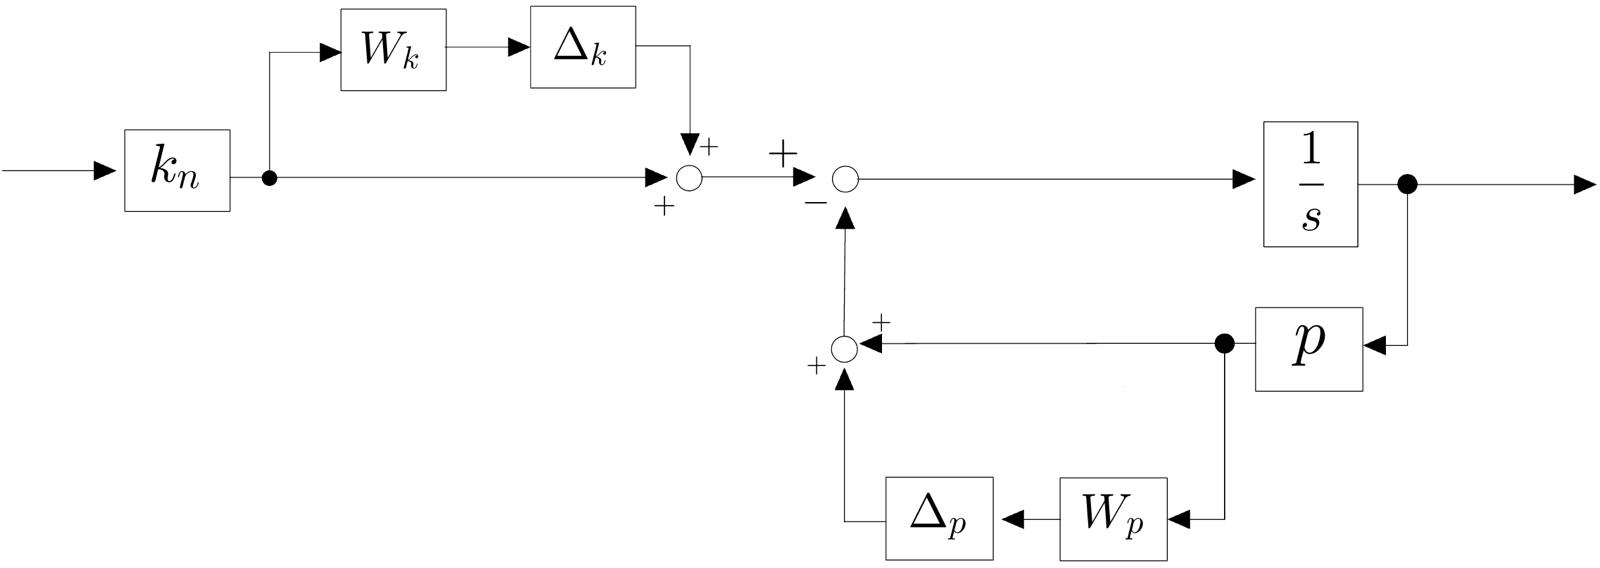
\includegraphics[scale=0.27]{img/ex1_mul.jpg}
    \caption{Block diagram for $G_p(s)$ (multiplicative set)}
    \label{fig:ex1_mul}
\end{figure}

\begin{figure}
    \centering
    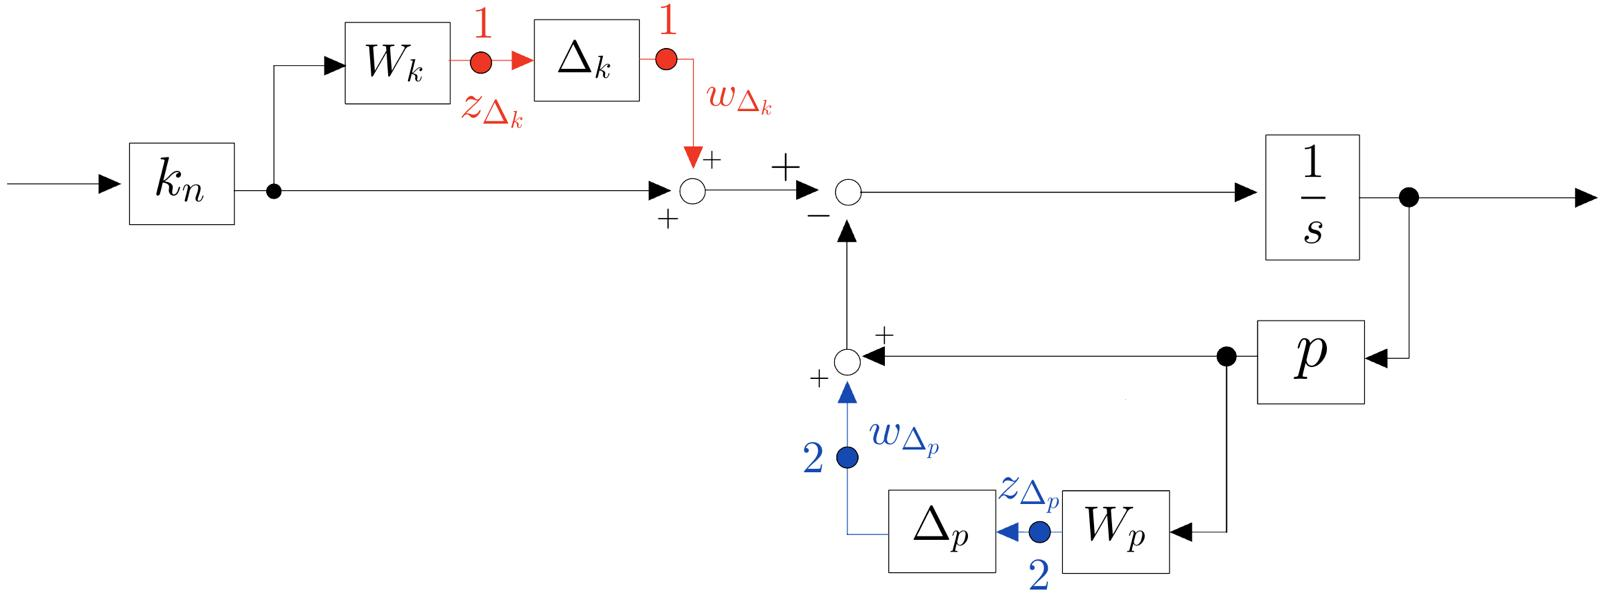
\includegraphics[scale=0.3]{img/ex2_num.jpg}
    \caption{Block diagram for $G_p(s)$ (multiplicative set) with numbered uncertainty channels}
\end{figure}

\newpage
\subsubsection*{Example 2 (model the reciprocal of an uncertain parameter)}
Given the following plant
\begin{equation}
    G_p(s)=\frac{k}{1+s\tau}, \quad     
\end{equation}
is required to find a block diagram description of it, in a way that can be implemented in a simulink scheme. 
\begin{multicols}{2}
    \noindent
    A rearragement of the terms is needed: 
\begin{equation}
    G_p(s)=k \ \frac{\frac{1}{s}\cdot \frac{1}{\tau}}{1+\frac{1}{s\tau}}
\end{equation}
We omit the gain, to focus our attention on the second part of the transfer function.

\newcolumn
The second term can be represented as:
\begin{center}
    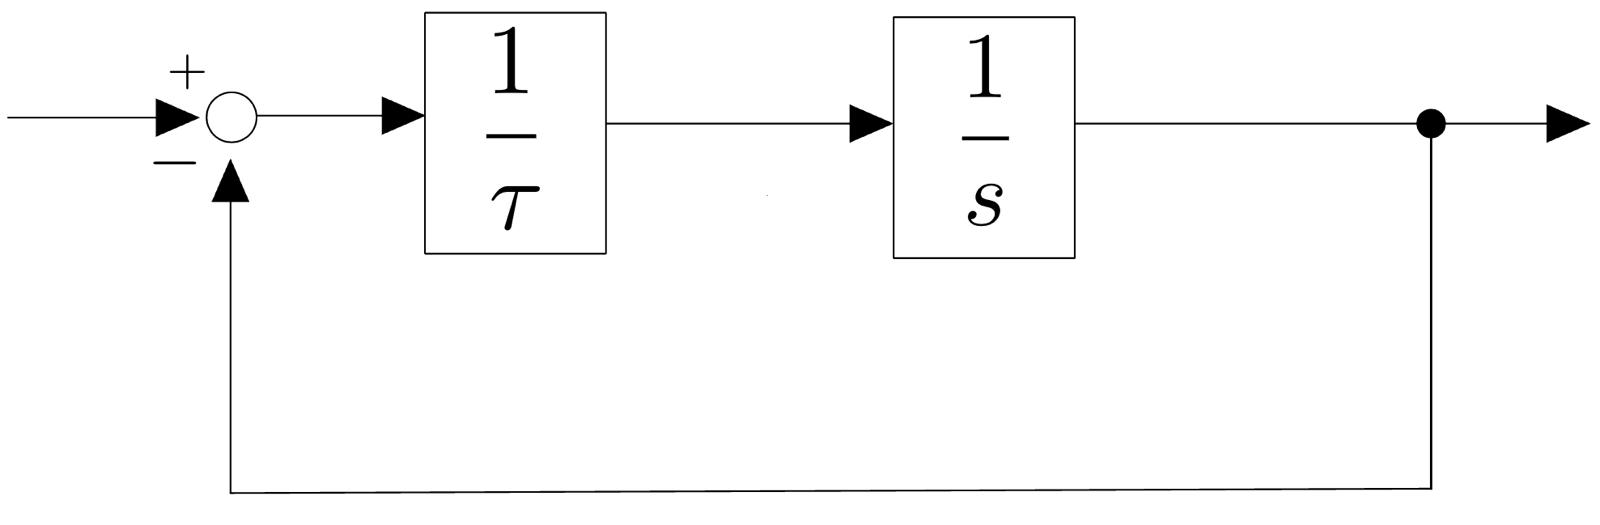
\includegraphics[scale=0.13]{img/tau.jpg}
\end{center}
\end{multicols}


\noindent
The second term can be recasted in a basic feedback structure whose direct path has the block $1/{s\tau}$, simply 1 in the feedback path. But how can we draw the diagram for the inverse of the uncertain parameter? It depends from the type of uncertainty set. 

\begin{multicols}{2}
    \noindent
\textbf{\textsf{Multiplicative set}}\\
The term $1/\tau$ can be written as:
\begin{equation}
    \frac{1}{\tau}=\frac{1}{\tau_n}\cdot
    \frac{1}{1+W_\tau \Delta_\tau}
\end{equation}
The related block diagram representation is:
\begin{center}
    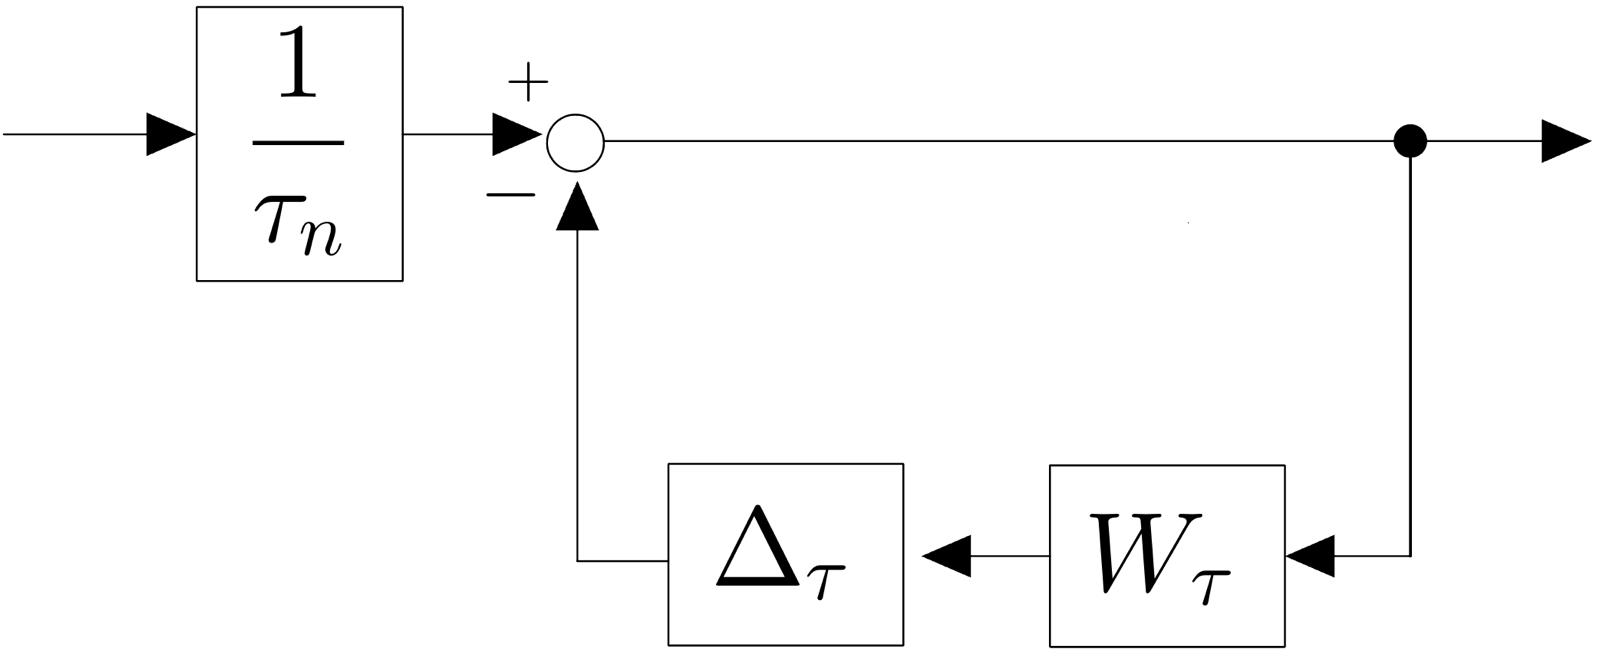
\includegraphics[scale=0.13]{img/tau_mul.jpg}
\end{center}

\newcolumn
\noindent
\textbf{\textsf{Additive set}}\\
The term $1/\tau$ can be written as:
\begin{equation}
    \frac{1}{\tau}=\frac{1}{\tau_n+W_\tau \Delta_\tau}=
    \frac{\frac{1}{\tau_n}}{1+\frac{W_\tau \Delta_\tau}{\tau_n}}
\end{equation}
The related block diagram representation is:
\begin{center}
    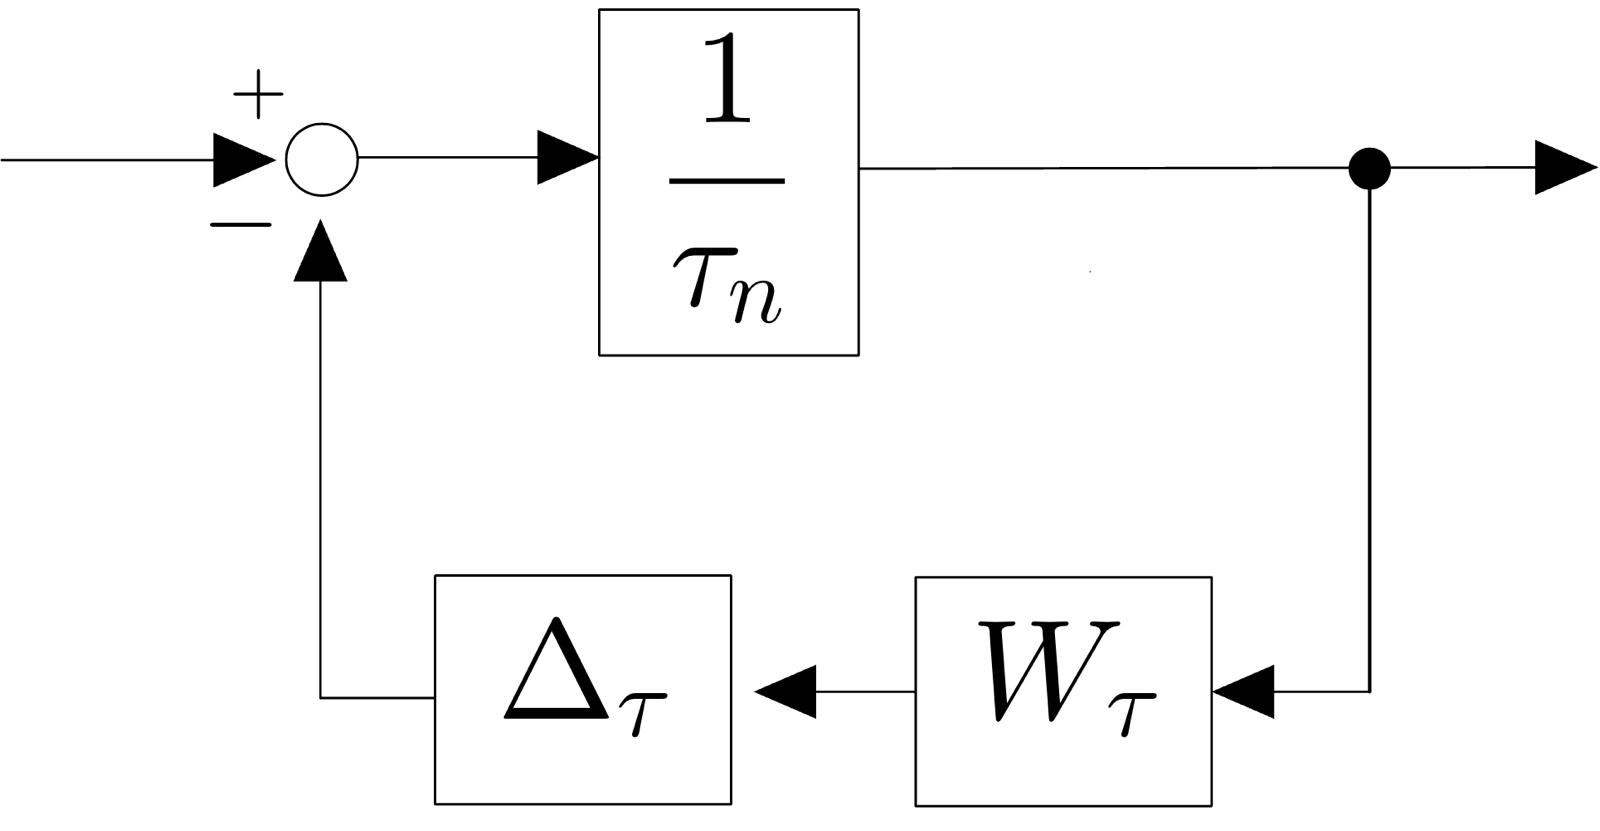
\includegraphics[scale=0.11]{img/tau_add.jpg}
\end{center}
\end{multicols}
\noindent
The remaining part of the discussion, about the port numbering and block $\Delta$ description, the way we retrieve $\Delta_\tau$ and $W_\tau$ does not change. This is the reason why we omit this part.
 
\subsubsection{Real pole in DC-gain form}
Here the objective is to analyze the block diagrams for the uncertain plant described by the following transfer function in \textit{DC-gain (or time constant) form}:
\begin{equation}\label{eq:ex2}
    G_p(s)=\frac{k}{1+\frac{s}{p}} \qquad
    \underline{k}\le {k} \le \overline{k}, \quad
    \underline{p}\le {p} \le \overline{p}
\end{equation}
\noindent

\begin{multicols}{2}
    \noindent
    Following the same path we algebrically manipulate the \Cref{eq:ex2} in order to obtain:
    \begin{equation*}
        G_p(s)=k \ \frac{\frac{p}{s}}{1+\frac{p}{s}}
    \end{equation*}
    \newcolumn
    \begin{center}
        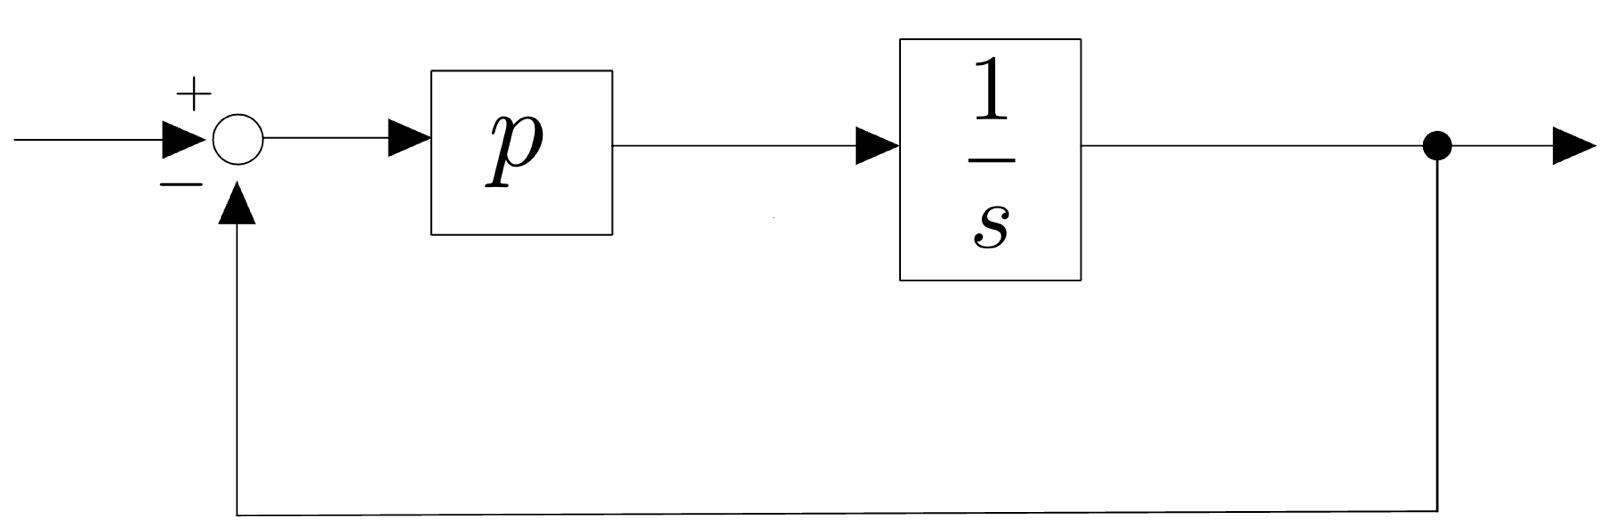
\includegraphics[scale=0.15]{img/ex2.jpg}
    \end{center}
\end{multicols}
\noindent
No other comments are needed  for modeling $p$ since it is a simple uncertain parameter whose modeling can follow the \Cref{tab:uncertainty_set}.


\subsubsection{Complex conjugate poles}
Given the following transfer function for an uncertain plant
\begin{equation}
    G_p(s)=\frac{k\omega_n^2}{s^2+2\zeta\omega_n{s}+\omega_n^2}\quad
    \underline{k}\le {k} \le \overline{k}, \quad
    \underline{\omega}_n\le {\omega_n} \le \overline{\omega}_n
\end{equation}
Here it is useful to apply the properties of the \textit{Laplace transform} in order to pass into a state-space description. In particular we know, by definition, that given a certain transfer function $G_p(s)$ it is defined as
\begin{align}
    &G_p(s)=\frac{y(s)}{u(s)} \iff y(s) (s^2+2\zeta\omega_n{s}+\omega_n^2)=u(s) \ k\omega_n^2 \iff \\
    &\frac{1}{\omega_n^2}\ddot{y}(t)+\frac{2\zeta}{\omega_n}\dot{y}(t)+y(t)=k{u(t)}\label{eq:diff_eq}
\end{align}
We can retrieve from the \textit{differential equation} \cref{eq:diff_eq} the state space description by introducing some state variables. In particular: 
\begin{align}
    x_1(t)=y(t) \quad
    x_2(t)=\dot{y}(t) \quad
\end{align}
Here we assume \textbf{zero initial conditions} so that we can write\footnote{
    Here the matrices of the state space description are: 
    \begin{equation*}
        A=\begin{bmatrix}
            0&1\\
            -\omega_n^2&-2\zeta\omega_n
        \end{bmatrix}, \quad 
        B=\begin{bmatrix}
            0\\
            k\omega_n^2
        \end{bmatrix}, \quad 
        C=[ 1 \quad 0]
    \end{equation*}
    Since they are not strictly necessary we put them here.
}:
\begin{equation*}
    \begin{cases}
        \dot{x_1}(t)=x_2(t)\\
        \dot{x_2}(t)=-2\zeta\omega_n{x_2}(t)-\omega_n^2{x_1}(t)+k\omega_n^2{u(t)}\\
        y=x_1
    \end{cases} \Longrightarrow \quad \begin{cases}
        \dot{x}(t)=Ax(t)+Bu(t)\\
        y(t)=Cx(t)
    \end{cases} 
\end{equation*}
In order to draw the block diagram we individuate the equation containing the $u(t)$ that is the input till reaching the output $y(t)$. The resulting block diagram is: 

\begin{figure}[h]
    \centering
    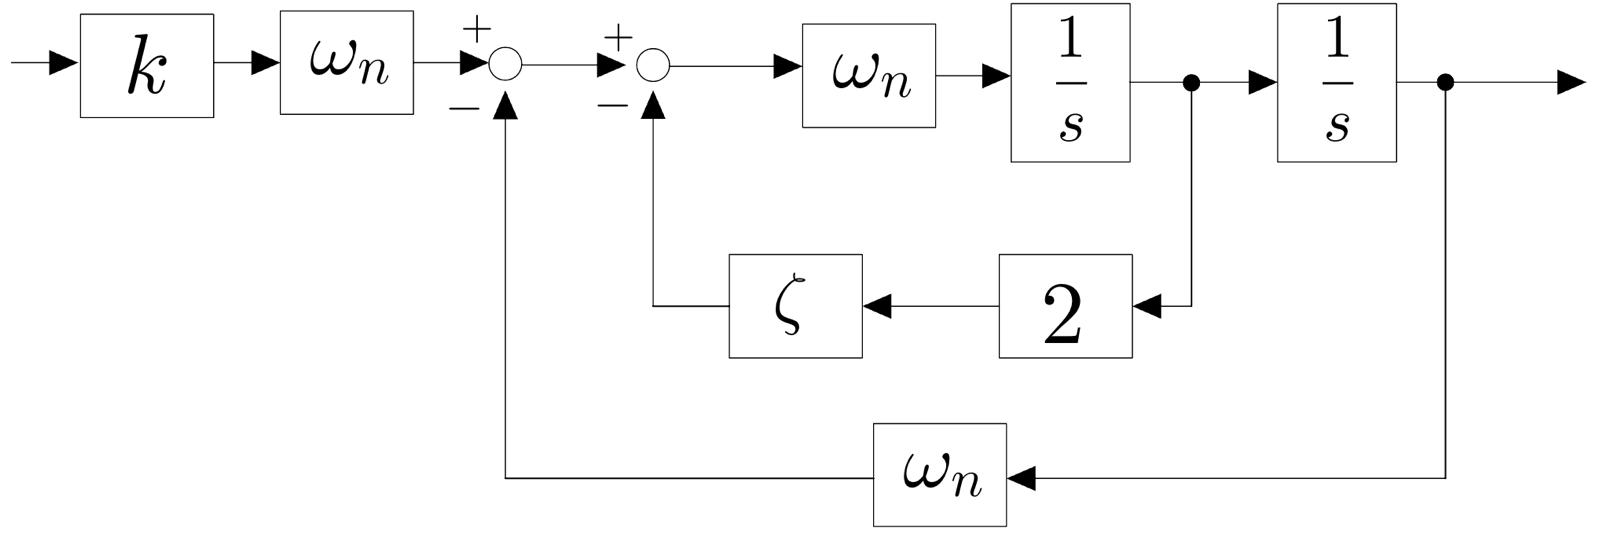
\includegraphics[scale=0.3]{img/complex_conj_plant.jpeg}
    \caption{Block diagram of $G_p(s)$}
\end{figure}
\newpage
\noindent
This is the general form of the transfer function containing the complex conjugate poles, the single parameters must be substituted with their own uncertain description using one of the uncertainty sets.\\
 This example is interesting since here there are repeated parameters, we can number with 1 the uncertainty related to the parameter $k$, 2 the uncertainty related to the damping factor $\zeta$, finally all the others are the uncertainty channels related to the natural frequency $\omega_n$. The resulting \texttt{deltaset} is
 
 \begin{equation}
    \texttt{deltaset}=[
        -1,0; \
        -1,0; \
        -2,0
    ]
 \end{equation}\\
\vspace{-1cm}
\hrule
\vspace{0.3em}
\noindent
\textsf{The description obtained so far by using the state space description is quite general, so that we could consider also the case of \textbf{non-zero} initial conditions. Clearly also the previous example would have been provided us with the possibility to follow the same appproach, however when simple manipulations can be algebraically done by using directly the transfer function it is more convient and fast.}

\section{Robust stability (RS) with structured uncertainty}
At this stage, since the controller is known, we can collapse the blocks $P$ and $G_c$ in a single one which we call $N$. Then, the structure we obtain can be called $N-\Delta$ (see \Cref{fig:NDelta}). In this context $N$ contains all the \textbf{known parts} of the feedback control system: the controller, actuators and nominal plant, the weighting functions accounting for the performance requirements.\\
This operation coincides with an \textit{upper linear fractional transformation (upper LFT)}, where we can write
\begin{equation}
    \begin{bmatrix}
        z_\Delta\\
        z_p
    \end{bmatrix}=\begin{bmatrix}
        N_{11}&N_{12}\\
        N_{12}&N_{22}
    \end{bmatrix}
    \begin{bmatrix}
        w_\Delta\\
        w_p
    \end{bmatrix}
\end{equation}
It can be prooved that ensuring robust stability for the $N-\Delta$ structure is equivalent to check that: 
\begin{equation}\label{eq:RS_cond}
    \det(I-N_{11}\Delta(j\omega))\ne0 \quad \forall \omega, \forall \Delta, \ \Vert \Delta \Vert_\infty<1
\end{equation}
where $N_{11}$ is the matrix tranfer function from $z_\Delta$ to $w_\Delta$. This equation comes from the generalized Nyquist stability criterion for MIMO systems. In this specific case such a condition is also called \textsf{determinant stability condition}. \emph{Note here that the performance channel are not involved.}

\newpage
\begin{multicols}{2}
    \begin{figure}[H]
        \centering
        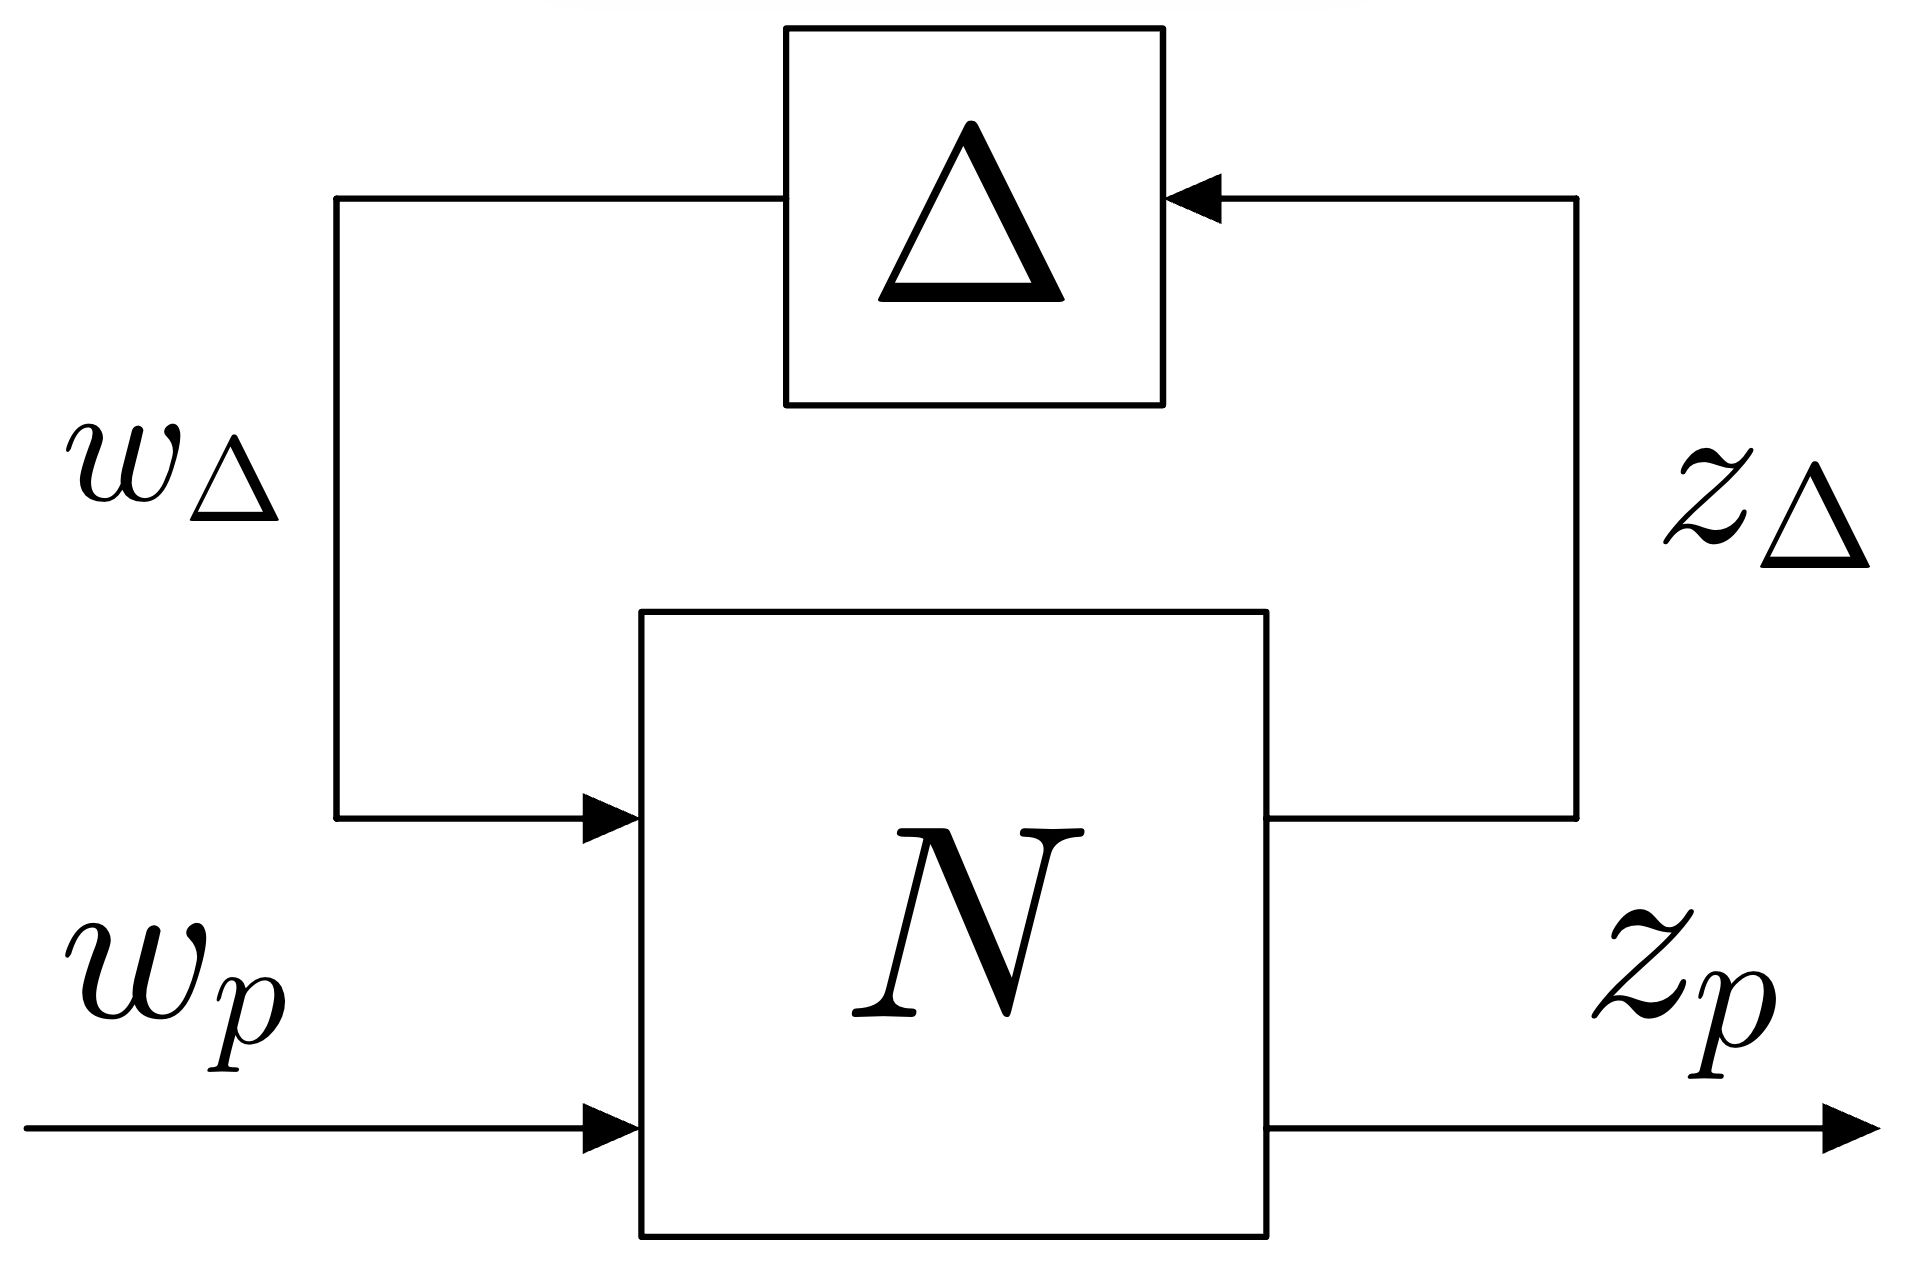
\includegraphics[scale=0.12]{img/NDelta.jpg}
        \caption{$N-\Delta$ structure for RS}
        \label{fig:NDelta}
    \end{figure} 
    \newcolumn
    \begin{figure}[H]
        \centering
        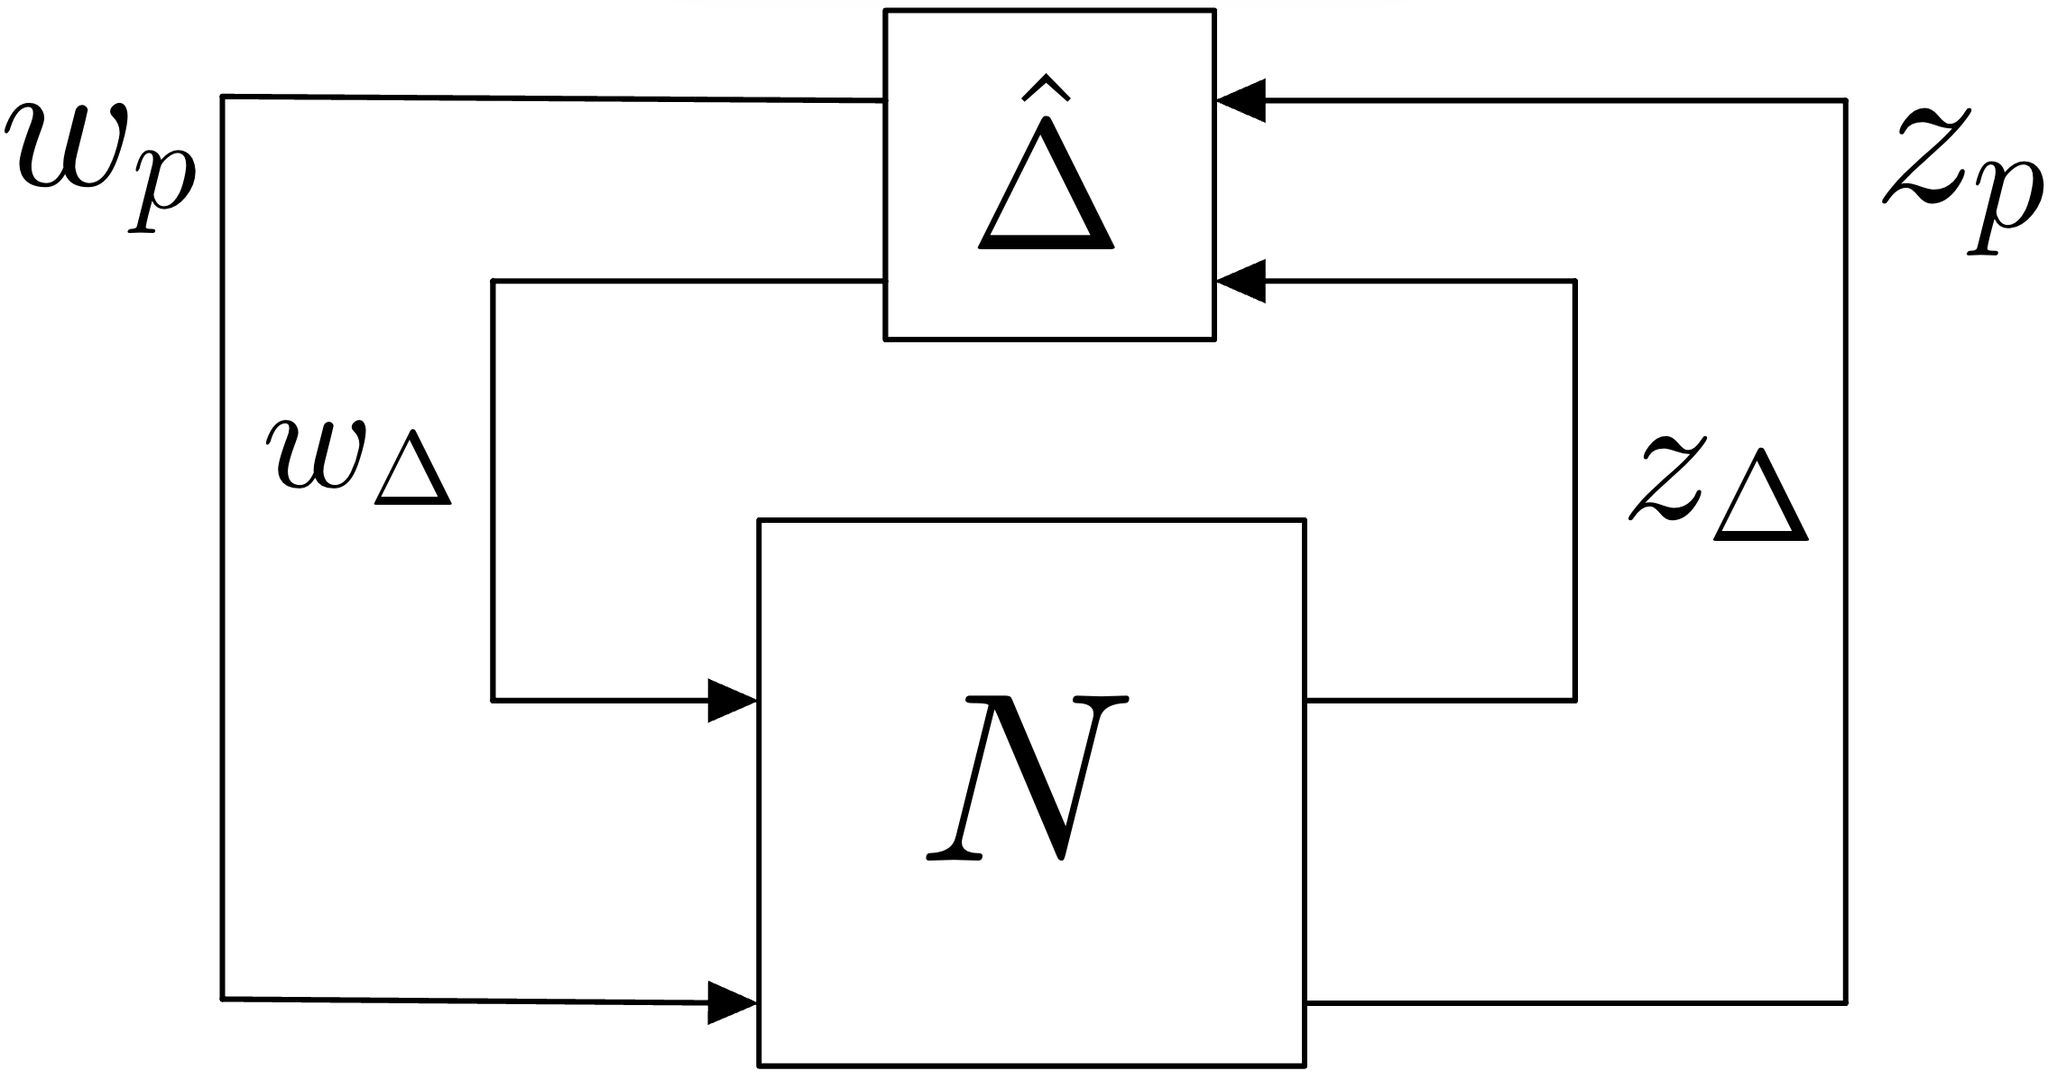
\includegraphics[scale=0.12]{img/NDeltahat.jpg}
        \caption{$N-\hat{\Delta}$ structure for RP}
    \end{figure}
\end{multicols}



\section{Robust performance (RP) with structured uncertainty}
In the context of robust control, robust performance requirements can be expressed as: 
\begin{equation}
    \Vert F(s,\Delta) \Vert_\infty<1, \quad \forall\Delta, 
\end{equation}
where $F(s,\Delta)$ is a given matrix transfer function accounting for the performance requirements, moreover it holds that $z_p=F(s,\Delta)w_p$. Such a functional $F$ can be written as: 
\begin{equation}
    F(s,\Delta)=\bigg\Vert
        \begin{matrix}
            W_S S(s,\Delta)\\
            W_T T(s,\Delta)
        \end{matrix}
    \bigg\Vert 
\end{equation}
Note that, differently from the case of \textit{nominal performances}, here the check is done on the original $S$ and $T$, the ones containing the uncertain plant instead of the nominal!
By using the properties of the LFT, can be shown that ensuring the robust performance in this case is equivalent to ensure the robust stability of the structure $N-\hat{\Delta}$ obtained by introducing a fictitious scalar complex uncertainty $\Delta_p$, which, in turn, is the same to require that:
\begin{equation}\label{eq:RP_cond}
    \det(I-N\Delta(j\omega))\ne 0 \quad \forall \omega, \forall \Delta
\end{equation}
Even in this case the \textit{determinant stability condition} derived from the generalized Nyquist Criterion is used.


\section{A tool to check robustness: structured singular value $\mu$}
The conditions in \Cref{eq:RS_cond} and \Cref{eq:RP_cond} we have just obtained are of little practical interest, since \textit{we cannot explore all the frequencies and all the uncertainties}, just to prove that the system is robust! An alternative, more practical, approach is needed. In particular, it may be useful to start by substituing in the determinant expression a certain $\Delta$ and to decrement it gradually. In particular: 
\begin{itemize}
    \itemsep-0.3em
    \item \textbf{Checking RS} is equivalent to compute the \textit{smallest structured uncertainty} $\Delta$ such that 
    \begin{equation}
        \det(I-N_{11}\Delta(j\omega))=0, \forall \omega
    \end{equation}
    \item \textbf{Checking RP} is equivalent to find the \textit{smallest structured uncertainty $\Delta$} such that the stability is destroyed, that is: 
    \begin{equation}
        \det(I-N\Delta(j\omega))=0, \forall \omega
    \end{equation}
\end{itemize}
At the end of the day:
\begin{itemize}
    \item If the smallest uncertainty is less than one, then the robust stability/robust performance is \textbf{not fulfilled} since the stability is broken for an allowed value of $\Delta$. In other words given our uncertain plant there are some values of the allowed uncertainty for which the robust requirement is 'destroyed'.
    \item If the smallest uncertainty is greater or equal than one, RS/RP is fulfilled, since such an uncertainty does not belong to the set of the allowed uncertainty.
\end{itemize}

\noindent
Such aspects can be better formalized by introducing: (i) a real scalar $k_m$ being the \textbf{singulatity margin}; (ii) the definition of a novel tool which will provide us with the possibility to check in an effective way RS/RP. This leads to the definition of the \textbf{structured singular value $\mu$}, that for the structure $N$, namely, is defined as:

\begin{equation}
    \large
    \mu(N,j\omega)=\frac{1}{\min\{k_m\in\mathbb{R}: \ \det(I-N(j\omega)\Delta(j\omega))=0, \ \Vert \Delta \Vert_\infty < 1\}}
\end{equation}
Note that $\mu(N,j\omega)$ is a real non-negative function of $\omega$, moreover since we take the inverse of the $k_m$ margin, robustness properties are guaranteed by the $\mu$ if such a value is, frequency by frequency, less than one.\\
Summarizing, here starting from the results related the determinant stability condition, we have introduced a tool by which we can check RS and RP in a systematic way.

\section{$\mu$-analysis}
We are are ready for give \textbf{necessary and sufficient} conditions for robust stability and robust performance in terms of $\mu$.\\
 Performing the \textbf{$\mu$-analysis} is the same to say that we are using the structured singular values in order to check Robust Stability/Robust Performance.

\begin{multicols}{2}
    \noindent\textsf{\textbf{ ROBUST STABILITY}}\\
    Assume that $G_c$ stabilizes $N$, the $N-\Delta$ structure is robustly stable if and only if
    \begin{equation}
        \mu(N_{11}, j\omega) < 1 \quad \forall \omega 
    \end{equation}
    
    \newcolumn
    \noindent
    \textsf{\textbf{ROBUST PERFORMANCE}}\\
    Assume that $G_c$ stabilizes $N$ (provides internal stability), the following conditions are equivalent: 
    \begin{itemize}
        \itemsep-0.3em
        \item $\Vert F(s,\Delta) \Vert_\infty < 1, \quad \Vert \Delta \Vert_\infty<1$  \ \textsf{(RP)}
        \item $\mu(N,j\omega)<1 \quad \forall \omega$ 
    \end{itemize}
\end{multicols}

\subsection{Tackling the complexity: $\mu_{ub}$, $\mu_{lb}$ bounds on the true $\mu$}
The results we have just given are very nice, except for the fact that computing the structured singular values is an \textbf{hard non-convex problem}, this is the reason why, practically speaking only some numerical upper and lower bounds $\mu_{ub}, \ \mu_{lb}$ on the real $\mu$ can be computed. On the contrary, computing such bounds results in a \textbf{convex optimization problem}.\\
Since, mostly we are not going to compute the real value for $\mu$, you can imagine that the conditions on the \textit{bounds of the true $\mu$} are no more necessary and sufficient.

\subsection{Sufficient conditions for robustness}
\begin{equation}
    \begin{cases}
        \underset{\omega}{\sup} \ \mu_{ub}(N_{11},\omega) < 1& \Longrightarrow \quad \textsf{ROBUST STABILITY}\\
        \underset{\omega}{\sup} \  \mu_{ub}(N,\omega) < 1 & \Longrightarrow \quad \textsf{ROBUST PERFORMANCE}
    \end{cases}
\end{equation}
This says us that if $\mu_{up}$ is less than one, RS/RP requirement is fulfilled, on the contrary if $\mu_{up}>1$ and $\mu_{lb}<1$ nothing can be said since the true $\mu$ might be greater than one, but also less than one.

\subsection{Necessary conditions for robustness}
\begin{equation}
    \begin{cases}
        \textsf{ROBUST STABILITY} & \Longrightarrow  \quad
        \underset{\omega}{\sup} \ \mu_{lb}(N_{11},\omega) < 1\\
        \textsf{ROBUST PERFORMANCE} & \Longrightarrow \quad
        \underset{\omega}{\sup} \ \mu_{lb}(N,\omega) < 1 
    \end{cases}
\end{equation}
Note that if $\mu_{lb} > 1$, then RS/RP are not fulfilled since the condition on the lower bound is a necessary one. The \Cref{tab:RSRP} summarizes all of these aspects.

\begin{table}[h]
    \centering
    \begin{tabular}{p{6cm} p{6cm} p{4cm}}
        \bottomrule[2pt]
        \textbf{ROBUST PERFORMANCE}& $\underset{\omega}{\sup} \ \mu_{ub}(N,j\omega)<1$& \textsf{fulfilled}\\
        & $\underset{\omega}{\sup} \ \mu_{lb}(N,j\omega)>1$ & \textsf{not fulfilled}\\
        & $\begin{cases}
            \underset{\omega}{\sup} \ \mu_{ub}(N,j\omega)>1\\
            \underset{\omega}{\sup} \ \mu_{lb}(N,j\omega)<1
        \end{cases}$ & \textsf{nothing can be said}\\
        \midrule[1pt]
        \textbf{ROBUST STABILITY}& $\underset{\omega}{\sup} \ \mu_{ub}(N_{11},j\omega)<1$&\textsf{fulfilled}\\
        & $\underset{\omega}{\sup} \ \mu_{lb}(N_{11},j\omega)>1$ & \textsf{not fulfilled}\\
        & $\begin{cases}
            \underset{\omega}{\sup} \ \mu_{ub}(N_{11},j\omega)>1\\
            \underset{\omega}{\sup} \ \mu_{lb}(N_{11},j\omega)<1
        \end{cases}$ & \textsf{nothing can be said}\\
        \bottomrule[2pt]
    \end{tabular}
    \caption{RP and RS checking by using $\mu_{lb}$ and $\mu_{ub}$}
    \label{tab:RSRP}
\end{table}

\vspace{-0.3cm}
    \noindent
    \textsf{At this point, we have all the ingredients in order to properly perform the $\mu$-analysis using upper and lower bounds on the real $\mu$. One important remark is that, in the case of RP, \textbf{one requirement at a time} must be checked. For example if we have to check performance requirements on different sinusoidal disturbances you have to perform the steps for $\mu$-analysis we are going to describe, considering them as 'separated'.
    }

\begin{table}[h]
    \centering
    \begin{tabular}{p{5cm} p{5cm} p{3cm} p{3cm}}
        \midrule[1.5pt]
        \textbf{Requirement}&\textbf{Constraint}&\textbf{Weight}&\textbf{Freq. range}\\
        \midrule
        $\vert e_{d_s}^\infty \vert \le \rho_s$, $d_s=a_s\sin(\omega_s{t})$&$\vert T(j\omega) \vert \le M_T^{HF} \ \forall \omega \ge \omega_s^{-}$&$W_{T\mu}=\frac{1}{M_T^{HF}}$&$[\omega_s,100\omega_s]$\\
        \midrule
        $\vert e_{d_p}^\infty \vert \le \rho_p$, $d_p=a_p\sin(\omega_p{t})$&$\vert S(j\omega) \vert \le M_S^{LF} \ \forall \omega \le \omega_p^{+}$&$W_{S\mu}=\frac{1}{M_S^{LF}}$&$[0.01\omega_p,\omega_p]$\\
        \midrule
        $\vert e_r^\infty \vert \le \rho_r$, $r(t)=\frac{R_0}{h!}{t^h}$& $\vert S^{*}(0) \vert \le k_{r} \ \omega \to 0, \ \nu\ge\nu_0$&$W_{S\mu}=s^{\nu_0+p} \cdot k_{r}$&$[10^{-8},10^{-3}]$\\
        \midrule
        $\vert e_{d_a}^\infty \vert \le \rho_a$, $d_a(t)=\frac{D_{a0}}{h!}{t^h}$& $\vert S^{*}(0) \vert \le k_{d_a} \ \omega \to 0, \ \nu\ge\nu_0$&$W_{S\mu}=s^{\nu_0+p} \cdot k_{d_a}$&$[10^{-8},10^{-3}]$\\
        \midrule
        $\vert e_{d_p}^\infty \vert \le \rho_p$, $d_p(t)=\frac{D_{p0}}{h!}{t^h}$& $\vert S^{*}(0) \vert \le k_{d_p} \ \omega \to 0, \ \nu\ge\nu_0$&$W_{S\mu}=s^{\nu_0+p} \cdot k_{d_p}$&$[10^{-8},10^{-3}]$
    \end{tabular}
    \caption{Guidelines for choosing the frequency range and weights on performances}
    \label{tab:guideline}
\end{table}

\newpage
\subsection{Robust performance - Constraining $T(s,\Delta)$}
Here two approaches to check robust performances on requirements constraining $T$ are presented. The first approach is the one using a \textbf{structured description} of the uncertainty, on the contrary the second approach is using the \textbf{unstructured} description of the uncertainty. Before entering into more details, keep in mind that by using this new technique we want to answer the following question:
\begin{center}
    \textbf{Is the complementary sensitivity function $T(s,\Delta)$ of our feedback control system satisfying a given requirement for 
    all of the realization of the uncertain plant $G_p$?}
\end{center}

\subsubsection{1st approach: structured description of the uncertainty}
\begin{enumerate}
    \itemsep-0.2em
    \item Build a new weighting function $W_{T\mu}$ (see \Cref{tab:guideline}) which only accounts for the requirement to check (this is a different weighting function, not the one has been built during the requirements translation); here $W_{T\mu}T$ is the transfer function between $w_p$ and $z_p$; 
    \item Build the \textit{generalized model} $N-\hat{\Delta}$ with the additional fictitious $\Delta_p$ uncertainty (eventually by pencil and paper)
    \item Accordingly to the previous point build a simulink scheme with input and output port properly numbered
    \item Compute the bounds\footnote{
        If the plots of the bounds on $\mu$ are very close, almost coincident, this is telling us that they are very close to the real $\mu$.
    } on $\mu(N,j\omega)$ in a range of frequency suitably chosen (see \Cref{tab:guideline}) and use \Cref{tab:RSRP} in order to draw conclusions on robustness.
\end{enumerate}

\subsubsection{Example}
\noindent
In the following there is an example of simulink scheme, all of the input/output ports related to the $\hat{\Delta}$ block are highlighted. The uncertain plant this scheme is related to is given: 
\begin{equation}
    G_p(s)=\frac{10^6{K}}{s^2+ps}, \quad 0.8\le{K}\le{1.2}; \quad
    420\le{p}\le{580}
\end{equation}
\vspace{-1cm}
\begin{figure}[h]
    \centering
    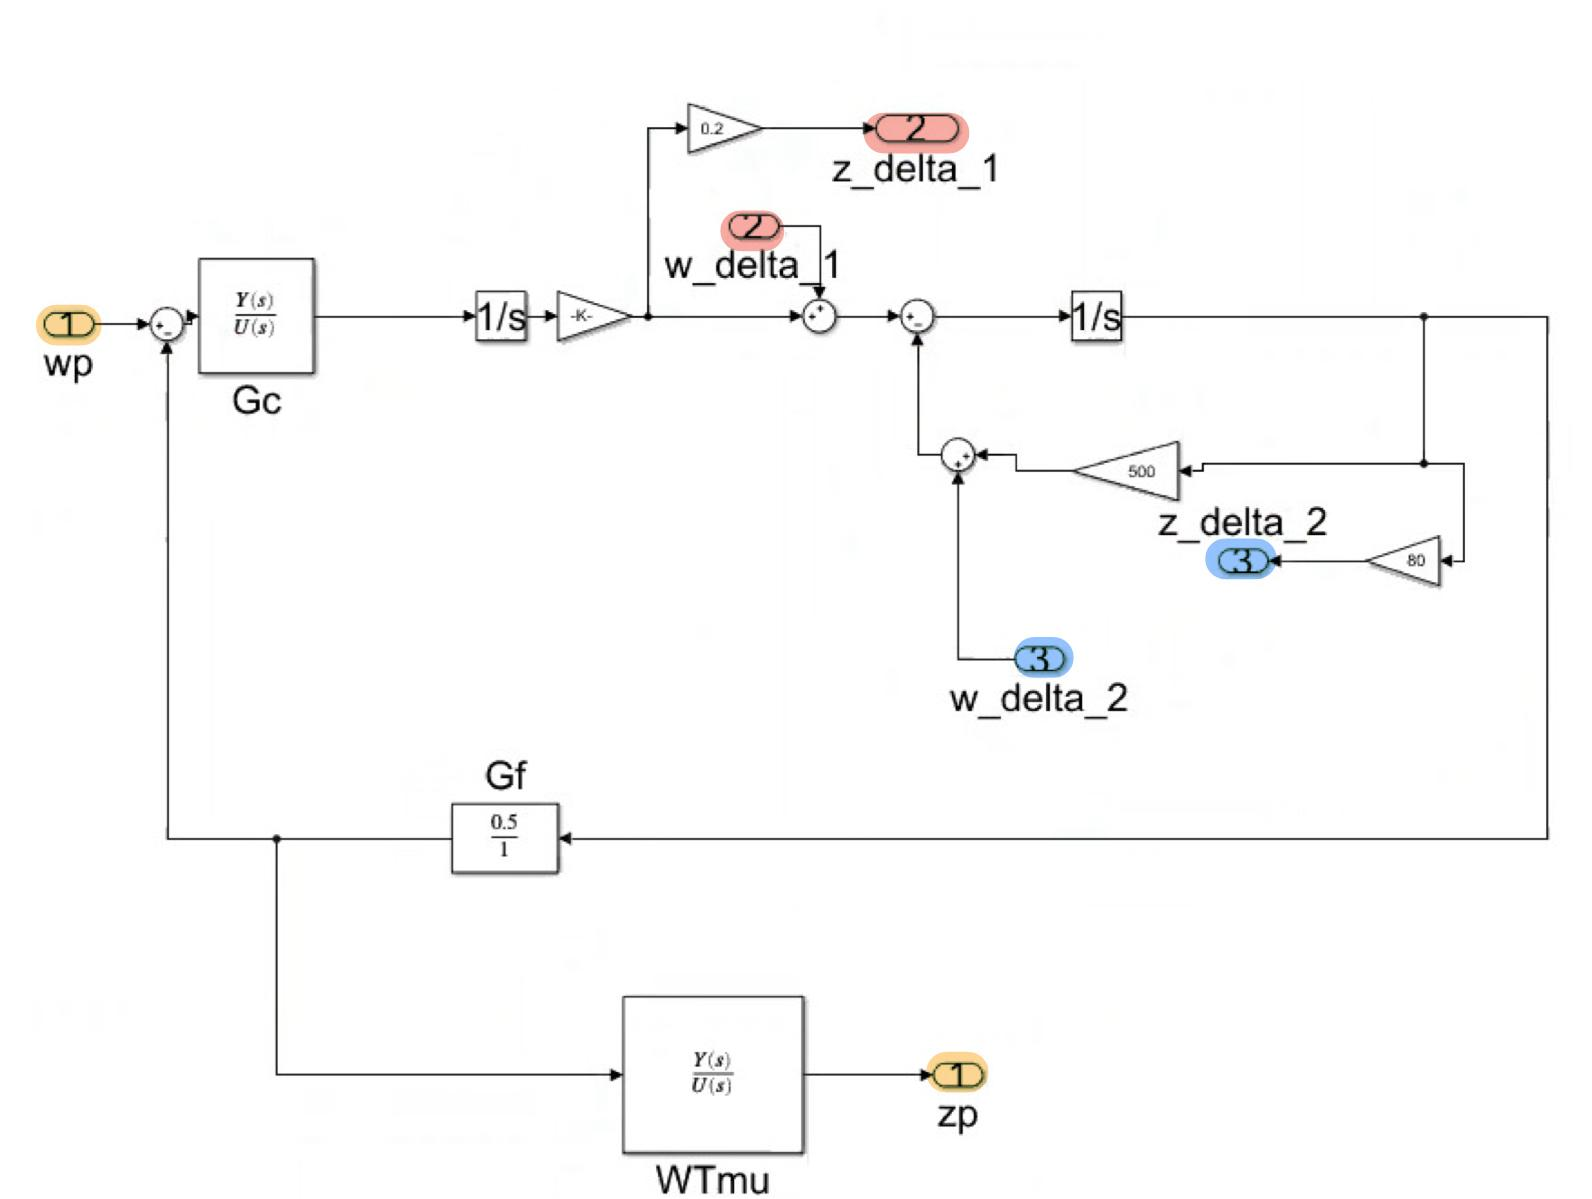
\includegraphics[scale=0.2]{img/EsNDeltaHat.jpg}
    \caption{Example: Simulink scheme of the $N$ structure}
\end{figure}

\noindent
The block diagonal matrix $\hat{\Delta}$ and the related describing \texttt{deltaset} array are:
\begin{equation*}
    \hat{\Delta}=\begin{bmatrix}
        {\color{orange}\Delta_p}&0&0\\
        0&{\color{red}\Delta_1}&0\\
        0&0&{\color{blue}\Delta_2}
    \end{bmatrix}, \quad 
    \texttt{deltaset}=[1,1; \ -1,0; \ -1,0];
\end{equation*}
where there is one complex uncertainty $\Delta_p$ and a couple of real uncertainties $\Delta_1$, $\Delta_2$.

\subsubsection{2nd approach: unstructured description of the uncertainty}
The only difference characterizing this alternative approach is that the scheme of $N$ contains a \textit{conservative} description of the uncertain plant $G_p(s)$ which uses (for example) the  \textit{multiplicative uncertainty} where it is described as belonging to the set
\begin{equation}
    M_m=\{
        G_p=G_{pn}(1+W_u\Delta), \ \Vert \Delta \Vert_\infty \le 1
    \}
\end{equation}
Finally, in the simulink scheme you have to replace the exact description of the plant with the different sources of uncertainty with a system with a \textbf{single complex scalar source}. Matrix $\hat{\Delta}$ and related \texttt{deltaset}, supposing that the position of the performance channel is unchanged, are: 
\begin{equation*}
    \hat{\Delta}=\begin{bmatrix}
        \Delta_p&0\\
        0&\Delta
    \end{bmatrix}, \quad
    \texttt{deltaset}=[1, 1; \ 1,1 ]
\end{equation*}

\noindent
\begin{remark}
    Also in this case the last step is to use the \Cref{tab:RSRP}. However, since the description of the plant $G_p(s)$ is a conservative one, whether robustness is not fulfilled with such a conservative description, nothing can be said and you must follow the first appproach! Otherwise, if robustness is fulfilled we can stop here our analysis because for sure the $N$ containing the exact description of the uncertainty will provide analog results. 
\end{remark}


\subsection{Robust performance - Constraining $S(s,\Delta)$}
What about requirements constraining $S$? As far as the first two approaches are concerned, analog steps must be followed. Again, performing the $\mu$-analysis for this type of requirements is giving us the answer to the question:
\begin{center}
    \textbf{Is the sensitivity function $S(s,\Delta)$ of our feedback control system satisfying a given requirement for 
    all of the realization of the uncertain plant $G_p$?}
\end{center}

\subsubsection{1st approach: structured description of the uncertainty}
The only difference with respect to the case of $T$ is that here the weighting function must be chosen is $W_{S\mu}$ and the picking point is changing. A structured description of the uncertainty is considered in the $N$ Simulink scheme.
\subsubsection{2nd approach: unstructured description of the uncertainty}
All unchanged except the description of the uncertain $G_p(s)$ which in this case is an \textit{unstructured} one. If the results of such an analysis are negative, the first approach must be used that is the best and most complete one.

\subsubsection{3rd approach: using the exact $\mu$}
This is a variant of the second approach, exploiting an important result: 

\begin{result}
When the uncertain plant is described in an unstructured fashion and the considered performance requirement is only providing constraints on $S(s,\Delta)$, the (exact) structured singular value $\mu(N,j\omega)$ can be computed as
\begin{equation}
    \mu(N,j\omega)=\big\vert \vert W_{S\mu}S_n\vert + \vert W_u T_n \vert \big\vert
\end{equation}
\end{result}
\noindent
Now, how to use this obtained function? 
\begin{equation*}
    \max_{\omega} \mu(N,j\omega) < 1 \Longrightarrow \textbf{Robust performance fulfilled}
\end{equation*}
Wheter such a condition is fulfilled, this is a very fast way to performing $\mu$-analysis on such requirements. However, if this is not the case, since the result is using a conservative description of the uncertainty, also in this case the first approach must be employed.



\subsection{Robust stability: changing the PUIs}
Till now, we have discussed $\mu$-analysis for checking robust performance. \textbf{What about Robust Stability?}
In this framework, the controller $G_c(s)$ is already designed with the objective of obtaining both Robust Stability and Nominal Performance fulfilled. \\
Then, given the description of the plant with the parameter uncertainty intervals (PUIs) a suitably designed weighting function $W_u$ is used, in order to check RS. At this point, it is not very interesting performing $\mu$-analysis using the original PUIs on which the $\mathcal{H}_\infty$ synthesis has been carried out: you are going to obtain a \textit{tautology}!\\

\noindent
Indeed, from a practical point of view, what is interesting is performing $\mu$-analysis on a \textbf{given range of frequencies using different intervals for the parameters}. The response of this procedure will be wheter the controller  is providing stability   for all the plants in the set generated by the new provided uncertainty intervals\footnote{
    It is remarkable, that this technique is also useful when you design the controller on a nominal plant, also using a different control design method (eg. Loop-shaping), and you want to know if such a controller provides stability when given parameters are ranging in certain intervals.
}. Also in this case there are two alternative approaches. 

\subsubsection{1st approach: defining the $N_{11}$ block}
Here the detailed structured description for the plant and for the entire FCS with related uncertainty is designed. What is changed are: (i) the nominal plant $G_{pn}$; (ii) the radius of the  parameters $W_{p}$ where $p$ indicates generically an uncertain parameter. Note that the extraction of $N_{11}$ starting from the Simulink scheme of $N$ is straightforward! The only thing is needed is the performance channels $z_p,\ w_p$ removal. \\
Don't loose ourself: no new weighting function is designed at this stage, since we are checking stability, not performance! At the end of the analysis the \Cref{tab:RSRP} can be used.

\subsubsection{2nd approach: defining a new weighting function $W_u^{\text{new}}$}
This approach is time consuming, but still valid to check Robust Stability on a different uncertainty set. This concerns with the design of a new weighting function $W_u^{\text{new}}$ using the newly provided PUIs, following the same guidelines we used during the controller design: we are seeking for a function $W_u^{\text{new}}$ that covers as tight as possible the cloud of curves representing the uncertainty set (eg. multiplicative).\\
After having built such a function the following condition must be checked: 
\begin{equation}
    \Vert W_u^{\text{new}} T_n \Vert_\infty < 1 \iff 
    \vert W_u^{-1,\text{new}}(j\omega) \vert > \vert T_n (j\omega)\vert \ \  \forall \omega
\end{equation}

\subsection{\textsc{Matlab} commands for $\mu$-analysis}
Whatever is the requirement for which you want to check RS/RP, the following \textsc{Matlab} commands (in the order they are described) must be used: 

\begin{table}[h]
    \centering
    \begin{tabular}{p{0.5cm} p{7cm} p{8cm}}
        \textbf{\#}&\textbf{Command}&\textbf{Description}\\
        \midrule[1.5pt]
        1&\texttt{[AN,BN,CN,DN]=linmod('N\_scheme')}&{Retrieves the state-space description of $N$ from the simulink model.}\\
        \midrule
        2&\texttt{Ns=minreal(zpk(ss(AN,BN,CN,DN)))}&{In order to make all the simplifications after numerical computations.}\\
        3&\texttt{[AN,BN,CN,DN]=ssdata(Ns)}&\\
        \midrule
        4&\texttt{N=pck(AN,BN,CN,DN)}&{Packs the information on $N$ in a way which is suitable for the $\mu$-toolbox.}\\
        \midrule
        5&\texttt{omega=logspace(low, down, \#points)}&{Builds the frequency range for which the computation on $\mu$ bounds is carried out. Good choice: \#points=1000}\\
        \midrule
        6&\texttt{Nf=frsp(N,omega)}&{Computes the frequency response of $N$ for the indicated omega range}\\
        \midrule
        7&\texttt{deltaset=[...;...;...]}&{Array describing the diagonal block matrix $\Delta$ or $\hat{\Delta}$} (according to the type of check we are doing)\\
        \midrule
        8&\texttt{[mubnds,d,s,p]=mu(Nf,deltaset)}&{Gives for the provided omega the values for lower and upper bounds. For further details see \texttt{help mu}}\\
        \midrule
        9&\texttt{vplot('liv,lm', mubnds)}&{Plots using log-scales the functions $\mu_{ub}(N,\omega)$ and $\mu_{lb}(N,\omega)$ }
        
    \end{tabular}
    \caption{\textsc{Matlab} commands for $\mu$-analysis}
    \label{tab:mu_commands}
\end{table}

\subsubsection{On the choice of \texttt{\#points} for \texttt{logspace}}
There is not a rule to choose the parameter \texttt{\#points} of the 5$^{th}$ command of the \Cref{tab:mu_commands}, however you can decide to improve the analysis in a given range of frequencies if you note that for example the value of one of the two bounds is very close to the threshold given by $1$. In that case an increased number of points in the specific range in which this occur can be useful in order to draw conclusions in the correct way.



\end{document}